\documentclass[12pt,a4paper]{article}
\usepackage[utf8]{inputenc}
\usepackage[spanish]{babel}
\usepackage[left=2cm,right=2cm,top=2cm,bottom=2cm]{geometry}
\usepackage{amsmath}
\usepackage{amsfonts}
\usepackage{amssymb}
\usepackage{lmodern}
\usepackage{amsmath}
\usepackage{enumerate}
\usepackage{algorithmic}
\usepackage{algorithm}
\usepackage{graphicx}
\usepackage{mathtools}

\newcommand{\LINECOMMENT}[1]{\STATE \(\triangleright\) #1}
\newcommand{\RESET}[1]{\STATE Reset: #1}
\def\BState{\State\hskip-\ALG@thistlm}

\begin{document}

\begin{titlepage}

  \begin{center}
    \vspace{15mm}
    \begin{Huge}
      Modelos y Simulación \\
      2017 \\
    \end{Huge}
  \end{center}

  \vspace{7mm}
  \begin{center}
    \begin{Large}
      \textbf{Trabajo Especial}
    \end{Large}
  \end{center}

  \vspace{20mm}
  \begin{Large}
    \begin{center}

        \textbf{Estudiantes:}

        \text{Scavuzzo, Juan Manuel}

        \text{Trucco, Francisco Carlos}
    \end{center}

  \end{Large}

\end{titlepage}


\tableofcontents

\section{\textbf{Introducción}}

    \par Se tiene un lavadero con una cierta cantidad de máquinas que deben
    estar funcionando en todo momento para que éste sea operativo. Dado
    que las máquinas se descomponen cada una cierta cantidad de tiempo,
    resulta relevante poder predecir el tiempo que tarda el sistema en fallar
    y determinar si es mejor aumentar la cantidad de máquinas de repuesto o
    aumentar la cantidad de operarios que las reparan.

    \par Claramente, determinar analíticamente el tiempo medio que tarda el
    sistema en fallar es muy dificil. Por esto es que se realizaron simulaciones
    para determinar el tiempo medio que transcurre hasta que el lavadero deja
    de ser operativo y la desviación estándar.

    \par Por otra parte, estas simulaciones permiten determinar si es más
    conveniente aumentar la cantidad de máquinas de repuesto o la cantidad de
    operarios.


    \subsection{Modelo}

    \par El lavadero cuenta con $N$ máquinas lavadoras en servicio y $S$
    máquinas de respuesto, todas ellas de idéntica marca, modelo y antigüedad.
    Además el lavadero cuenta con los servicios de técnicos que reparan
    las máquinas cuando éstas se rompen. Los técnicos trabajan en paralelo y
    cada uno se encarga de arreglar máquinas de a una por vez.
    Todos los tiempos de funcionamiento de las máquinas hasta descomponerse
    son variables aleatorias independientes exponenciales con un tiempo medio de
    fallar de $T_f$.
    El tiempo de reparación de una máquina que ingresa al taller es una
    variable exponencial con tiempo medio igual a $T_r$, independiente de todos
    los anteriores.

    \par Se dice que el sistema falla cuando se tiene menos de $N$ máquinas
    funcionando en un momento dado o, equivalentemente, cuando posee más de $S$
    máquinas defectuosas en el taller de reparación.

    \par Para resolver el problema en cuestión, se desarrolló un algoritmo que
    simula la relación que se establece entre los lavarropas que se rompen,
    aquellos que se están arreglando y los lavarropas de repuesto hasta que el
    sistema falla.
    En esta simulación se considera un \textbf{evento} cuando se rompe una máquina
    o cuando se termina de arreglar una.
    Entonces, si se rompe una máquina, y no puede ser atendida por el
    técnico porque éste está arreglando otra, ésta se considera en la cola de
    espera para ser atendida. Una vez que un operario termina de arreglar un
    máquina, o bien comienza a reparar otra o bien se considera libre.


\pagebreak

\section{Algoritmo y descripción de las variables}

    \par En este trabajo se desarrolló un algoritmo que
    generaliza la idea de el problema propuesto. El algoritmo retorna el tiempo
    que pasa hasta que el sistema deja de ser operativo, dada una cantidad
    arbitraria de técnicos reparadores, máquinas de repuesto y máquinas que deben
    estar funcionando en todo momento.

    \subsection{Parámetros del Algoritmo}

        \par Los parámetros del algoritmo son:
        \begin{itemize}
            \item{$N$: Cantidad de máquinas que deben estar funcionando en todo
              momento.}
            \item{$S$: Cantidad de máquinas de repuesto.}
            \item{$T_f$: Tiempo medio de falla de una máquina.}
            \item{$T_r$: Tiempo medio de reparación de una máquina por un
              operador.}
            \item{$O$: Cantidad de operadores que reparan las máquinas.}
        \end{itemize}

        \par Tanto el tiempo de falla de una máquina como el tiempo que tarda un
        operario en arreglar una máquina, tienen distribución exponencial con
        media $T_f$ y $T_r$ respectivamente.


    \subsection{Variables internas del Algoritmo}

        Por otro lado, se utilizaron las siguientes variables:
        \begin{itemize}
            \item{$t$: Tiempo actual.}
            \item{$failure\_times$: Lista de los tiempos de fallos de máquinas.}
            \item{$fix\_times$: Lista de los tiempos en los que se finalizan los
              arreglos de las máquinas.}
            \item{$fixing$: Cantidad de operarios que están arreglando
              máquinas o equivalentemente, la cantidad de máquinas que están
              siendo arregladas.}
            \item{$broken$: Cantidad de máquinas que están rotas (incluye
              aquellas que están siendo arregladas).}
        \end{itemize}

    \begin{algorithm} [H]
    \caption{Simulation($N$, $S$, $O$, $T_f$, $T_r$)}
    \label{alg}
    \begin{algorithmic} [1]
    \STATE $ t \coloneqq  0 $
    \STATE $ broken \coloneqq  0 $
    \STATE $ fixing \coloneqq  0 $
    \STATE $ failure\_times \coloneqq \lbrack  \mathcal{E}(1/T_f)_0, \dots , \mathcal{E}(1/T_f)_{N-1} \rbrack $
    \STATE $ fix\_times \coloneqq  \lbrack \infty_0, \dots, \infty_{O-1}\rbrack $

    \WHILE{$ broken \leq S $}
    \IF{$ failure\_times_0 < fix\_times_0 $}

      \STATE $ t \coloneqq failure\_times_0$
      \STATE $ broken \coloneqq broken + 1 $

      \IF{$ broken \leq S $}
        \STATE $ failure\_times \coloneqq \lbrack X_1, \dots, X_{N-1}, t +
         \mathcal{E}(1/T_f)\rbrack $
        \STATE Sort $ failure\_times $
      \ENDIF

      \IF{$ broken > fixing $ and $ fix\_times_{N-1} = \infty $}
        \STATE $ fix\_times \coloneqq \lbrack Y_0, \dots, Y_{O-2}, t + \mathcal{E}(1/T_r)\rbrack $
        \STATE Sort $ fix\_times $
      \ENDIF

    \ELSE

      \STATE $ t \coloneqq fix\_times_0 $
      \STATE $ broken \coloneqq broken - 1 $
      \STATE $ fixing \coloneqq fixing - 1 $

      \IF{$ broken = fixing $}
        \STATE $ fix\_times \coloneqq \lbrack Y_1, \dots, Y_{O-1}, \infty \rbrack $
      \ENDIF

      \IF{$ broken > fixing $}
        \STATE $ fix\_times \coloneqq \lbrack Y_1, \dots, Y_{O-1}, t + \mathcal{E}(1/T_r)\rbrack $
        \STATE $ fixing \coloneqq fixing + 1 $

      \ENDIF
      \STATE Sort $ fix\_times $

    \ENDIF
    \ENDWHILE
    \RETURN $ t $
    \end{algorithmic}
    \end{algorithm}

    \par El algoritmo mantiene dos listas ($ failure\_times$ y $fix\_times $)
    con los tiempos de los eventos ordenados de menor a mayor. Dado que están
    ordenadas, $ min(failure\_times_0, fix\_times_0) $ representa el próximo
    evento que ocurrirá. Los tiempos de falla se inicializan con valores
    generados a partir de una variable aleatoria exponencial con media $T_f$.
    Los tiempos de reparación se inicializan todos en infinito dado que no
    existen lavarropas en reparación.

    \par La simulación del lavadero se realiza hasta que éste deje de funcionar,
    es decir hasta que la cantidad de máquinas descompuestas sea mayor a la
    cantidad de máquinas de repuesto i.e., $ broken > S $.

    \par Si se descompone un lavarropas, se lo reemplaza por uno de repuesto y
    se calcula para este último el momento en el que fallará. Además, si un
    operario está libre comenzará a arreglar el lavarropa; por lo que también se
    calcula el tiempo que tardará.

    \par Si un operario termina de arreglar un lavarropas y hay un lavarropas
    descompuesto, se pone a trabajar inmediatamente y se calcula el tiempo que
    tardará en completar su tarea. Si no hay un lavarropas descompuesto, se
    marca al operario como libre. Para indicar que está libre se actualiza su
    tiempo a infinito. Esto significa que el próximo evento relacionado con la
    finalización de una reparación realizada por este operario nunca ocurrirá.

\pagebreak


\pagebreak

\section{Resultados}

    \par En todos los casos, se realizaron 10000 simulaciones para calcular la media
    y la desviación estándar. Con los resultados de estas simulaciones se
    contruyeron los distintos histogramas que se presentan a continuación.

    \par Dado el contexto del problema, resulta de gran interés saber cómo maximizar el
    tiempo que tarda el sistema en fallar. Para ésto, los parámetros más
    significativos son $S$ y $O$ ya que éstos son los que el dueño del
    local modficaría para maximizar sus ganancias.
    Es por ésto que los parámetros que se pusieron en comparación son los
    anteriormente nombrados.

    \par Los tres experimentos realizados utilizaron los siguientes parámetros:
        \begin{itemize}
            \item{2 máquinas de repuesto y 1 operario.}
            \item{2 máquinas de repuesto y 2 operarios.}
            \item{3 máquinas de repuesto y 1 operario.}
        \end{itemize}

    \par En los histogramas, el eje X representa el tiempo, en meses, en el que falla el
    sistema y el eje Y representa la frecuencia del tiempo que tarda el sistema en
    fallar.
    En la esquina superior derecha se puede observar la media y la desviación
    estándar resultante los experimentos.
    Adicionalmente, se muestran a continuación:
        \begin{itemize}
            \item{\underline{Para $S = 2$ y $O = 1$:}
                    $ \overline{X}(n) = 1.779 $ meses y $ \sqrt{S^2(n)} = 1.583 $ meses}
            \item{\underline{Para $S = 2$ y $O = 2$:}
                    $ \overline{X}(n) = 2.606 $ meses y $ \sqrt{S^2(n)} = 2.512 $ meses}
            \item{\underline{Para $S = 3$ y $O = 1$:}
                    $ \overline{X}(n) = 3.614 $ meses y $ \sqrt{S^2(n)} = 3.320 $ meses}
        \end{itemize}


\pagebreak

    \subsection{Comparación: Agregar un operario}

    \par En este caso, realizamos una comparación de la situación en que el lavadero
    tiene 2 máquinas de repuesto y 1 sólo operario con la situación en que tiene 2
    máquinas de repuesto y 2 operarios.
    Se ejecutó el algoritmo antes descripto con los dos conjuntos de parámetros
    correspondientes a las situaciones a comparar. Esto es:

    \[
      N = 5; \; T_F = 1; \; T_R = 0.125; \; S = 2; \; O = 1
    \]
    \[y\]
    \[
      N = 5; \; T_F = 1; \; T_R = 0.125; \; S = 2; \; O = 2
    \]

    \begin{figure}[h]
        \centering
        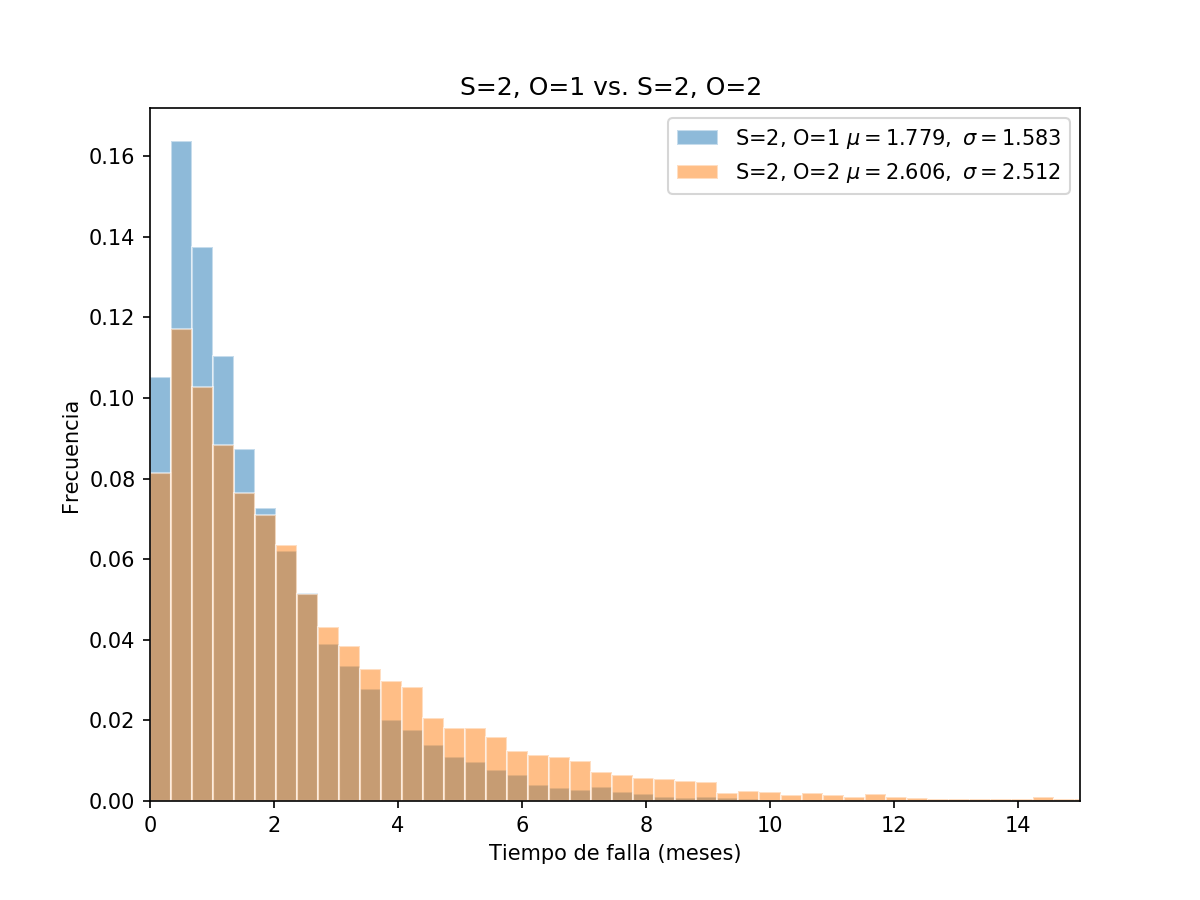
\includegraphics[scale=0.8]{images/S2O1vsS2O2.png}
        \caption{Histograma de comparación entre S = 2, O = 1 y S = 2, O = 2}
        \label{fig:S2O1vsS2O2}
    \end{figure}
    \vspace{5mm}

    \par En la Figura \ref{fig:S2O1vsS2O2} se puede observar que cuando se agrega un
    operario el tiempo esperado de falla
    del sistema aumenta considerablemente. Este resultado es el que esperábamos, pues
    aumenta la velocidad de reparación de máquinas al aumentar la cantidad de individuos
    capaces de reparar al mismo tiempo.

    \pagebreak

    \subsection{Comparación: Agregar una máquina}

    \par En este caso, realizamos una comparación de las tres situaciones antes
    mencionadas.
    \par Se ejecutó el algoritmo antes descripto con los conjuntos de parámetros
    correspondientes a las situaciones a comparar. Esto es:

    \[
      N = 5; \; T_F = 1; \; T_R = 0.125; \; S = 2; \; O = 1
    \]
    \[y\]
    \[
      N = 5; \; T_F = 1; \; T_R = 0.125; \; S = 3; \; O = 1
    \]


    \begin{figure}[h]
        \centering
        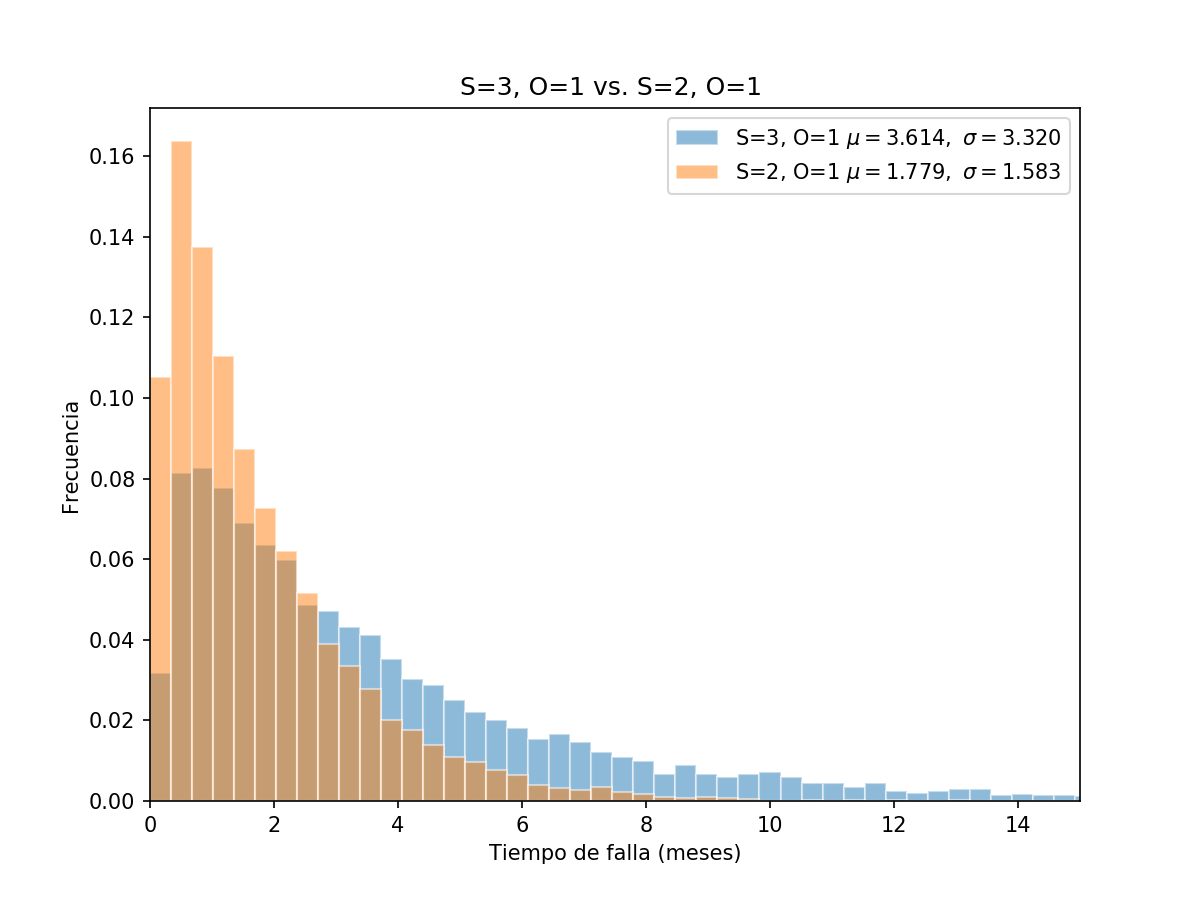
\includegraphics[scale=0.8]{images/S3O1vsS2O1.png}
        \caption{Histograma de comparación entre S = 2, O = 1 y S = 3, O = 1.}
        \label{fig:S2O1vsS3O1}
    \end{figure}
    \vspace{5mm}


    \par En la Figura \ref{fig:S2O1vsS3O1} se puede observar que cuando se agrega una
    máquina el tiempo esperado de falla
    del sistema aumenta considerablemente. Este resultado es el que esperábamos, pues al
    aumentar la cantidad de máquinas de repuesto los operarios tienen más tiempo para
    reparar las máquinas antes de que el sistema falle.

  \pagebreak

  \subsection{Comparación: Agregar una máquina vs. agregar un operario}

  \par En este caso, realizamos una comparación de la situación en que el lavadero
  tiene 3 máquinas de repuesto y 1 sólo operario con la situación en que tiene 2
  máquinas de repuesto y 2 operarios.
  Se ejecutó el algoritmo antes descripto con los dos conjuntos de parámetros
  correspondientes a las situaciones a comparar. Esto es:

  \[
    N = 5; \; T_F = 1; \; T_R = 0.125; \; S = 3; \; O = 1
  \]
  \[y\]
  \[
    N = 5; \; T_F = 1; \; T_R = 0.125; \; S = 2; \; O = 2
  \]

  \begin{figure}[h]
      \centering
      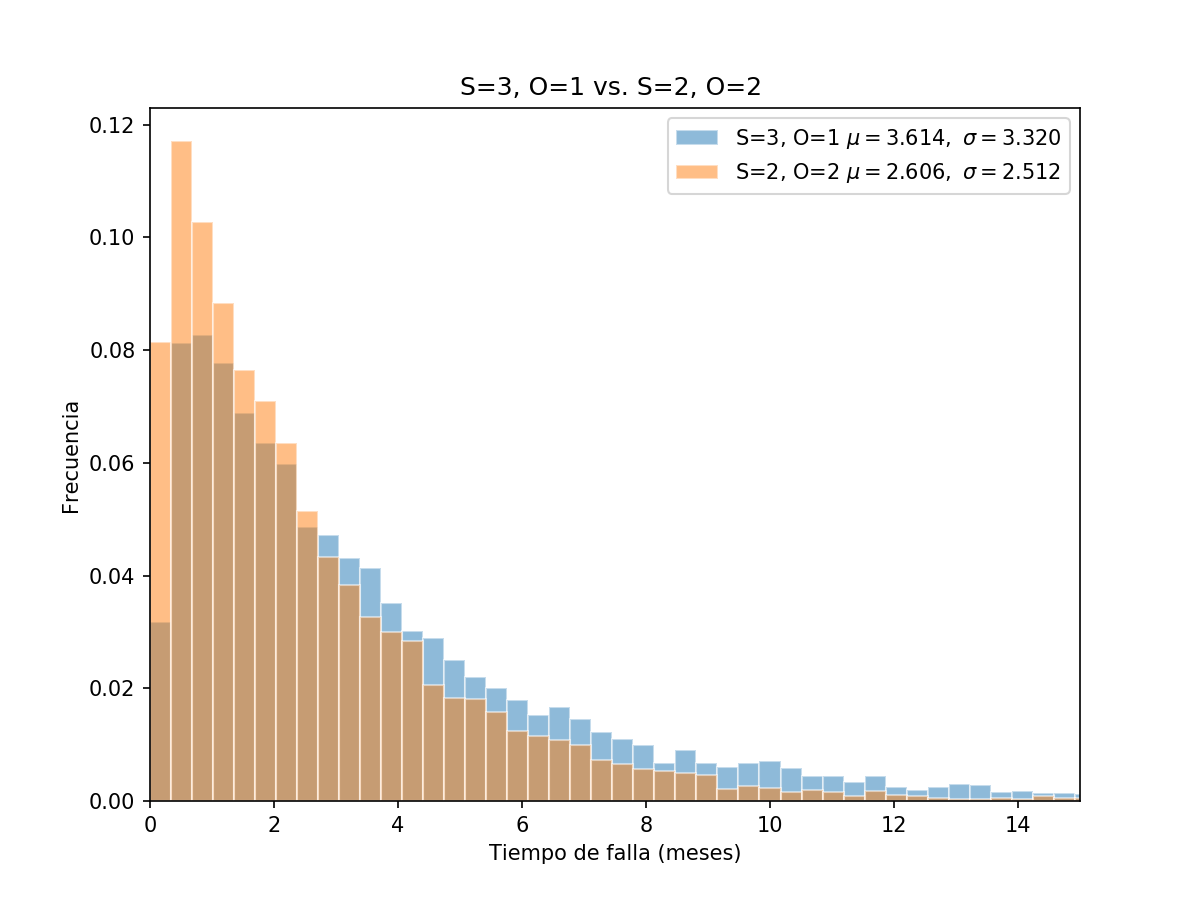
\includegraphics[scale=0.8]{images/S3O1vsS2O2.png}
      \caption{Histograma de comparación entre S = 3, O = 1 y S = 2, O = 2}
      \label{fig:S3O1vsS2O2}
  \end{figure}
  \vspace{5mm}

  \par En la Figura \ref{fig:S3O1vsS2O2} se puede observar que adquirir una máquina más
  de repuesto es más conveniente
  que contratar un operario extra pues el tiempo medio de falla del sistema aumenta.
  En particular, se puede notar en el histograma que la probabilidad de que el sistema falle
  dentro de los primeros 2 meses es considerablemente superior en el caso de que
  se contrata a un nuevo operario.


\pagebreak

\section{Conclusión}

    \par Se presentó el problema de determinar el tiempo de falla esperado de un lavadero
    en función de la cantidad de operarios y lavarropas de repuesto. Se construyó un
    modelo y a partir del mismo se obtuvieron datos simulados correspondientes al
    tiempo de falla del sistema. Dado que resulta de gran interés saber cómo
    maximizar el tiempo que tarda el sistema en fallar en función de estos
    parámetros, los distintos experimentos realizados varían estos parámetros.


    \par Agregar una máquina de repuesto incrementa el tiempo medio de fallo del sistema
    en un 50\%. Agregar un operario incrementa el tiempo medio de fallo del sistema
    en un 107\%. Claramente, agregar una máquina aumenta más el tiempo medio de fallo
    del sistema que agregar un operario. Estos resultados no deben extrapolarse a
    otras situaciones en las cuáles los parámetros sean distintos (ver Resultados).

    \par Es importante destacar que el algoritmo propuesto puede ser útil para realizar
    otros experimentos modificando los parámetros del mismo.


\pagebreak

\end{document}
